\chapter{Защита технических систем и микроприборов от вибрационных и ударных воздействий}

\section{Техническое задание}

Дано:
\begin{itemize}
    \item схема расположения ВИ:
        \begin{itemize}
            \item координаты $y_1  = y_2  = 70~мм$;
            \item координаты $z_1  = -z_2 = 70~мм$;
            \item координаты $y_3  = y_4  = -60~мм$;
            \item координаты $-z_3 = z_4  = 60~мм$;
        \end{itemize}
    \item масса $m = 3~кг$ (вес $G = 30~Н$);
    \item коэффициент демпфирования $\xi = 0.3$.
    \item степень жёсткости внешних воздействий:
        \begin{itemize}
            \item нижняя граница частоты возбуждающей вибрации $f_{н} = 30~Гц$;
            \item верхняя граница частоты возбуждающей вибрации $f_{в} = 500~Гц$;
            \item виброускорение вибрации $a_0 = 6g$;
            \item длительность ударного импульса $\tau = 4~мс$;
            \item амплитуда ударного импульса $a = 15g$.
        \end{itemize}
\end{itemize}

Задача: рассчитать систему виброизоляторов (ВИ) блока технических систем (ТС) с установленными выше параметрами.

\begin{figure}[!h]
    \centering
    \begin{subfigure}[b]{0.45\textwidth}
        \centering
        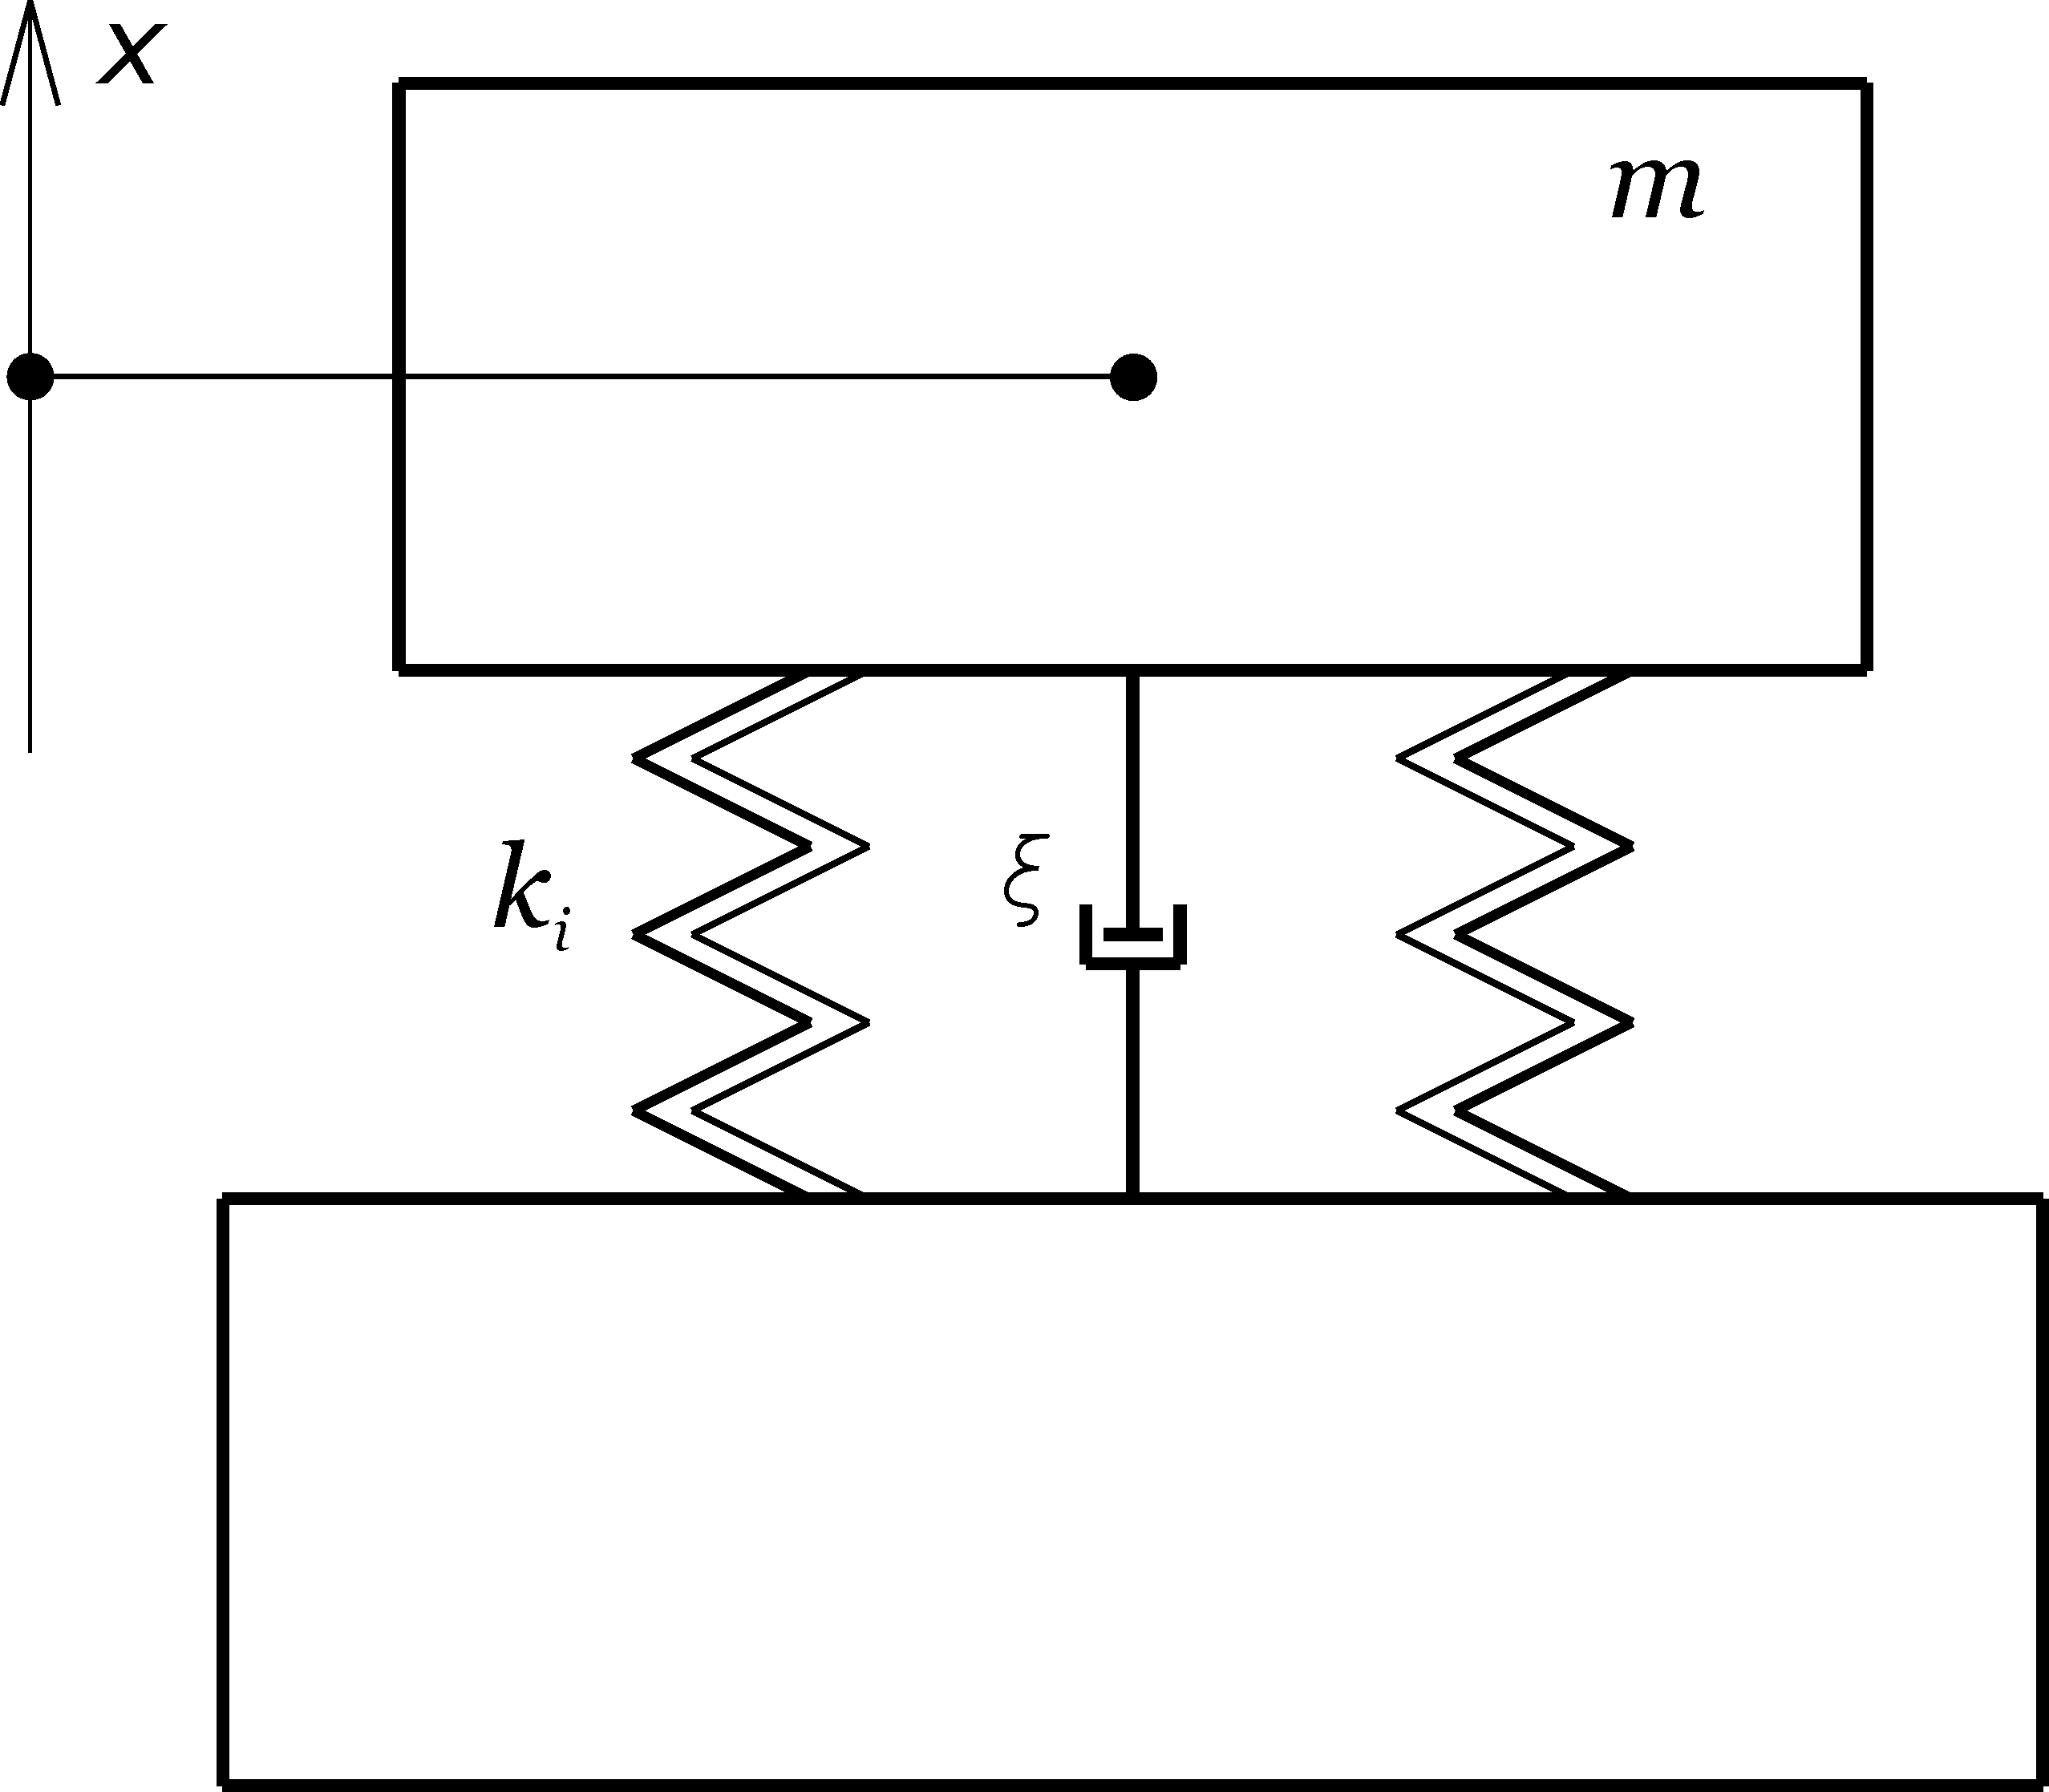
\includegraphics[width=\textwidth]{component-sideview.pdf}
        \caption{} 
        \label{fig:component-sideview}
    \end{subfigure}
    \begin{subfigure}[b]{0.45\textwidth}
        \centering
        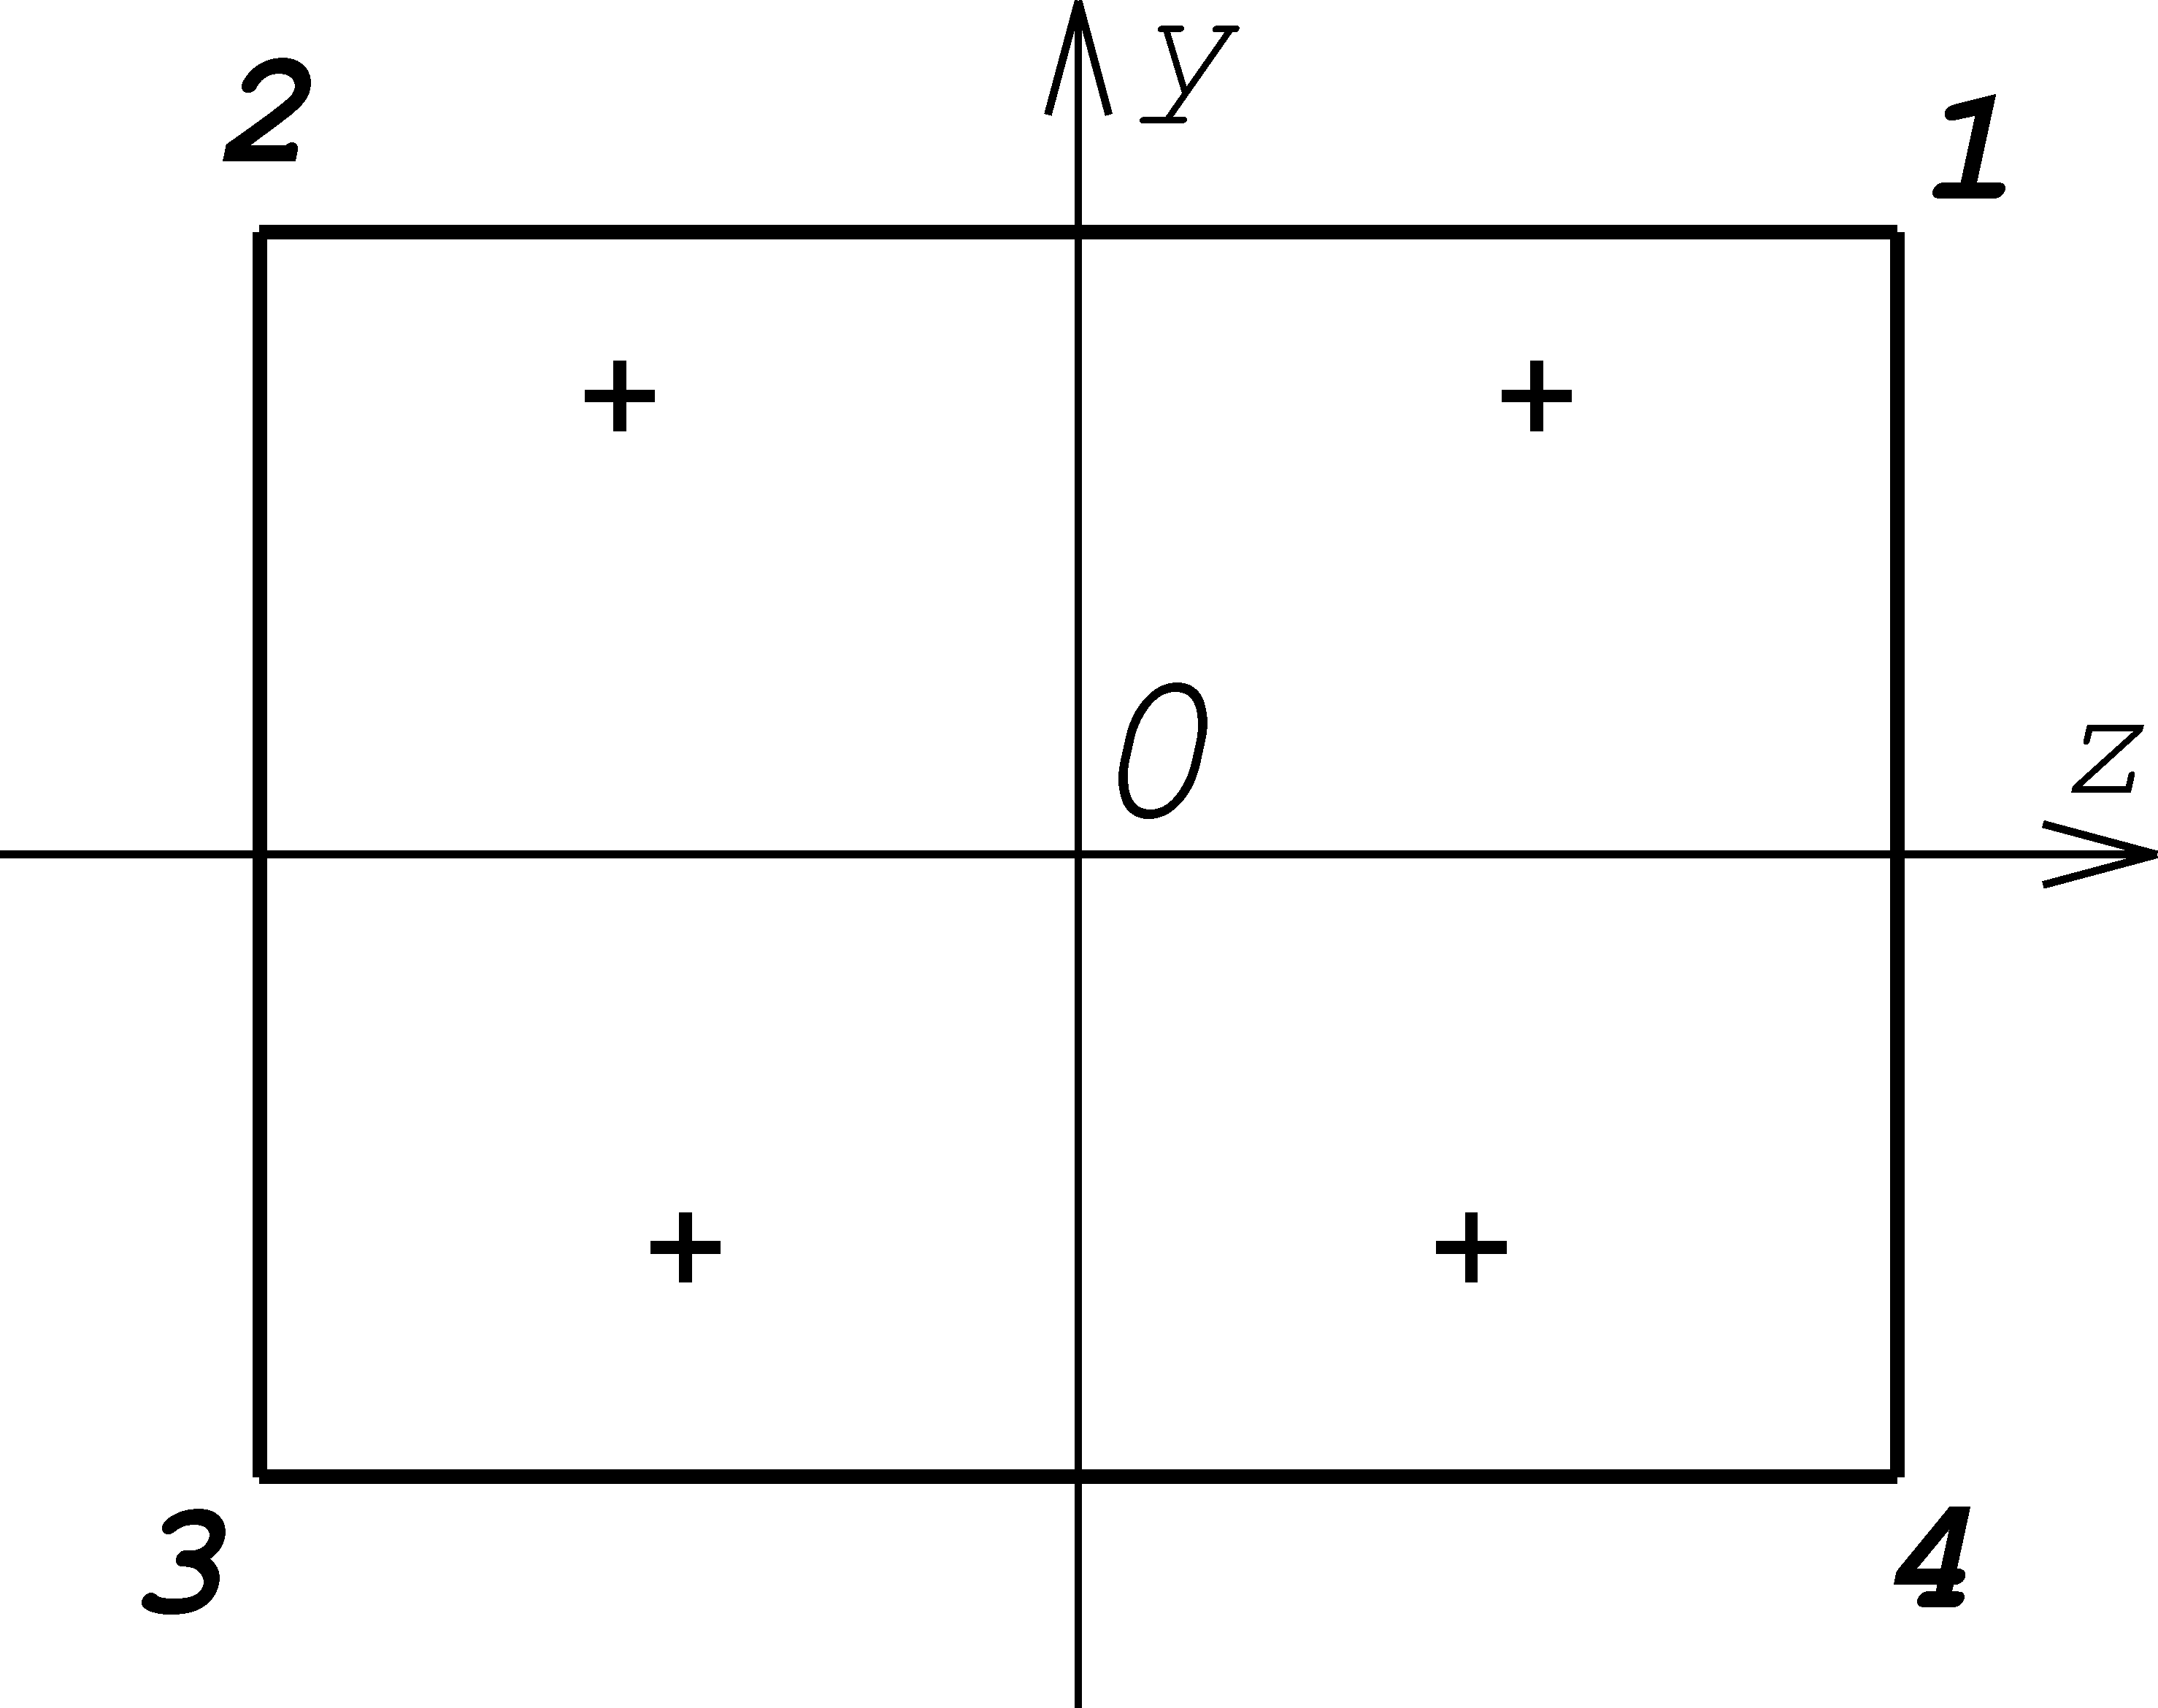
\includegraphics[width=\textwidth]{component-topview.pdf}
        \caption{}
        \label{fig:component-toview}
    \end{subfigure}
    \caption{Система виброизоляторов:
        а "--- вид сбоку;
        б "--- вид сверху.
    }
    \label{fig:component}
\end{figure}

\section{Решение}

\subsection{Статический расчёт системы ВИ}
1. Определим предварительно максимальную амплитуду вибрации основания:
\[
    A_{осн} = \frac{a_0}{\omega_{Н}^2}
            = \frac{6g}{(2 \pi f_{н})^2}
            = \frac{6 \cdot 10000}{(2 \pi 30)^2}
            = 1.7~мм.
\]

2. Для определения статических нагрузок используем уравнения:
\begin{align*}
    P_1 + P_2 + P_3 + P_4 - G = 0; \\
    P_1 z_1 + P_2 z_2 + P_3 z_3 + P_4 z_4 = 0; \\
    P_1 y_1 + P_2 y_2 + P_3 y_3 + P_4 y_4 = 0.
\end{align*}

С учётом симметрии расположения ВИ система уравнений приобретает вид:
\begin{equation*}
    \begin{cases}
        2 P_1   + 2 P_3   = G; \\
        y_1 P_1 - y_3 P_3 = 0. 
    \end{cases}
\end{equation*}
Решая СЛАУ, находим $P_1 = P_2 = \frac{90}{13} \approx 6.92~Н$ и $P_3 = P_4 = \frac{105}{13} \approx 8.08~Н$.

Выполним проверку:
\[
    2 P_1 + 2 P_3 = 2 \cdot 6.92 + 2 \cdot 8.08 
                  = 30
                  = G.
\]

3. Так как $\max \limits_i P_i~=~8.08~Н$, то выберем марку ВИ~АПН-1 с номинальной нагрузкой $P_{ном} = 5\==10~Н$ и жёсткостью по основной оси $k_x = 6.8~Н/мм$.

4. Определим статическую осадку ВИ:
\begin{align*}
    \Delta_1 = \Delta_2 = \frac{P_1}{k_x} = \frac{6.92}{6.8} \approx 1.02~мм; \\
    \Delta_3 = \Delta_4 = \frac{P_3}{k_x} = \frac{8.08}{6.8} \approx 1.19~мм.
\end{align*}
Для выравнивания блока используем прокладки толщиной
\[
    \delta = \Delta_3 - \Delta_1 = 1.19 - 1.02 = 0.17~мм.
\]

\subsection{Динамический расчёт системы ВИ}
1. Рассчитаем эквивалентную жёсткость системы ВИ:
\[
    K_{\sum} = \sum \limits_{i = 1}^n {k_x}_i
             = 4 k_x
             = 4 \cdot 6.8
             = 27.2~Н/мм
             = 27.2 \cdot 10^3~Н/м.
\]

2. Рассчитаем частоту собственных колебаний системы ВИ:
\[
    f_0 = 0.159 \sqrt \frac{K_{\sum}}{m}
        = 0.159 \sqrt \frac{27.2 \cdot 10^3}{3}
        = 15.1~Гц.
\]

3. Рассчитаем коэффициенты амортизации по формуле
\[
    K_{А} = \frac{\sqrt{1 + (2 \xi \nu)^2}}{\sqrt{(1 - \nu^2)^2 + (2 \xi \nu)^2}}
\]
и представим в виде таблицы (табл. \ref{tab:amortisation_coeffs}).

\begin{table}[!h]
    \centering
    \caption{Зависимость коэффициента амортизации $K_{А}$ от коэффициента рассогласования $\nu$.}
    \label{tab:amortisation_coeffs}
    \begin{tabular}{|l|c|c|c|c|c|c|c|c|}
        \hline
        $\nu$  & 0    & 0.5  & 1    & 1.4  & 2    & 3    & 4    & 5    \\ \hline
        $K_{А}$  & 1.00 & 1.29 & 1.94 & 1.02 & 0.48 & 0.25 & 0.17 & 0.13 \\ \hline
    \end{tabular}
\end{table}

По данным из табл. \ref{tab:amortisation_coeffs} строим АЧХ (рис. \ref{fig:frequency-response}).

\begin{figure}[!h]
    \centering
    \begin{tikzpicture}
        \begin{axis}[
            title={АЧХ},
            xlabel={Коэффициент рассогласования $\nu$},
            ylabel={Коэффициент амортизации $K_{А}$},
            xmin=0,
            xmax=5,
            ymin=0,
            xmajorgrids=true,
            ymajorgrids=true,
            ]

            \addplot[
            smooth,
            color=blue,
            mark=*,
            ]
            coordinates{
                (0, 1.00)
                (0.5, 1.29)
                (1, 1.94)
                (1.4, 1.02)
                (2, 0.48)
                (3, 0.25)
                (4, 0.17)
                (5, 0.13)
            };

            % \node[right] at (axis cs: 1.1, 2){$(1, 1.94)$};
        \end{axis}
    \end{tikzpicture}
    \caption{АЧХ.}
    \label{fig:frequency-response}
\end{figure}

4. Определяем максимальную амплитуду колебаний блока на низшей частоте вибраций $f_{н} = 30~Гц$ при $\nu = \frac{f_{н}}{f_0} = \frac{30}{15.1} \approx 2.0$ и $K_{А} = 0.5$:
\[
    A_{вын} = K_{А} \cdot A_{осн}
    = 0.5 \cdot 1.7
    = 0.85~мм.
\]

Максимальное ускорение, действующее внутри блока, составит:
\[
    a_{\max} = K_{А} \cdot a_0
    = 0.5 \cdot 6g
    = 3g.
\]

% 5. Из графика АЧХ (рис. \ref{fig:frequency-response}) видно, что виброизоляция достигается во всём диапазоне частот вибрации.
5. Так как $A_{вын} = 0.85~мм < \min\limits_i \Delta_i = \Delta_1 = 1.02~мм$, то выбранный тип ВИ обеспечит защиту блока от заданной вибрации.

\subsection{Расчёт системы ВИ на действие удара}
1. Рассчитаем условную частоту ударного импульса:
\[
    \omega_{у}
    = \frac{\pi}{\tau}
    = \frac{\pi}{4 \cdot 10^{-3}}
    \approx 785.4.
\]
и коэффициента расстройки:
\[
    \nu
    = \frac{\omega_{у}}{\omega_0}
    = \frac{785.4}{2 \pi \cdot 15.1}
    \approx 8.3.
\]

2. Определим коэффициент передачи удара:
\[
    K_{у}
    = \frac{2 \nu}{\nu^2 - 1} \cos \frac{\pi}{2 \nu}
    = \frac{2 \cdot 8.3}{8.3^2 - 1} \cos \frac{\pi}{2 \cdot 8.3}
    = 0.24.
\]

3. Определим амплитуду ускорения аппарата:
\[
    \ddot{x}_{\max}
    = a \cdot K_{у}
    = 15 g \cdot 0.24
    = 3.6 g.
\]

4. Определим максимальное относительное перемещение:
\[
    x_{\max}
    = \frac{a \cdot K_{у}}{\omega_0^2}
    = \frac{3.6 g}{\left(2 \pi \cdot 15.1\right)^2}
    = \frac{3.6 \cdot 10000}{\left(2 \pi \cdot 15.1\right)^2}
    \approx 4.0~мм.
\]

Вывод: так как $x_{\max} = 4.0~мм > \min\limits_i \Delta_i = \Delta_1 = 1.02~мм$, то выбранный тип виброизолятора не обеспечит защиту блока от заданного ударного воздействия.
